\usetikzlibrary{patterns}
\usetikzlibrary{decorations.pathmorphing}
\usepackage{titlesec,calc}
% \renewcommand{\familydefault}{\sfdefault}

\titleformat{\section}[hang]
{\normalfont\bfseries}
{\thesection.}{0.5em}{}
 \titlespacing{\section}{0pt}{3pt}{0pt} % Horizontal space, before space, after space

\mode<presentation>
{
  \usetheme{CambridgeUS}
  \usecolortheme{whale}
  \usecolortheme{lily}

  \setbeamercovered{transparent}
  \usefonttheme[onlymath]{serif}
}

\title[Pendulum Model] % (optional, use only with long paper titles)
{\large \course: \coursename \\[5pt] \semesteryear\\[5pt] Pendulum Robot Model}

\subtitle
{} % (optional)

\author[\instructorshort]% (optional, use only with lots of authors)
{\instructorlong\credits}
%{T. Vincent\inst{1} \and S.~Another\inst{2}}
% - Use the \inst{?} command only if the authors have different
%   affiliation.

\institute[\instituteshort] % (optional, but mostly needed)
{\institutelong}


\date % (optional)
{}



% If you have a file called "university-logo-filename.xxx", where xxx
% is a graphic format that can be processed by latex or pdflatex,
% resp., then you can add a logo as follows:

%\pgfdeclareimage[height=1.1cm]{university-logo}{UniversityLogo}
%\logo{\pgfuseimage{university-logo}}



% Delete this, if you do not want the table of contents to pop up at
% the beginning of each subsection:
%\AtBeginSection[]
%{
%  \begin{frame}<beamer>{Outline}
%    \tableofcontents[currentsection,currentsubsection]
%  \end{frame}
%}


% If you wish to uncover everything in a step-wise fashion, uncomment
% the following command:

%\beamerdefaultoverlayspecification{<+->}



\begin{document}
\maketitle
 
\section{Full Pendulum model}

To design a controller for the balancing pendulum, it will be useful to have a simulation model to test your designs. A picture of of a two-wheeled robot and an idealized description is shown below.  The robot is approximated as a two-mass pendulum, with angle $\phi$ defining the tilt, and $x$ defining the translational position of the base of the robot. The force $f$ and torque $\tau_{m}$ is due to the motors acting on the wheels.

\begin{figure}[h]
\begin{center}
\includegraphics[height=2.5in]{Graphics/robot}\hspace{1in}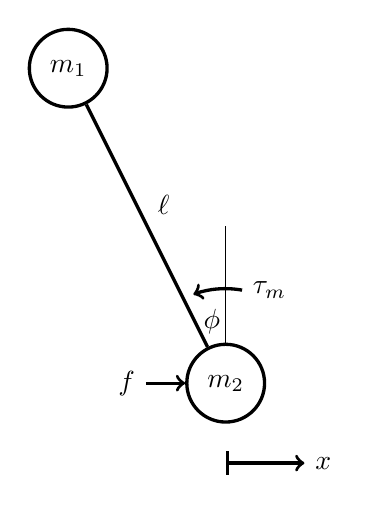
\begin{tikzpicture}[very thick,
sysblock/.style={draw,rectangle,inner sep=6pt,minimum width=1.5cm,minimum height=1.2cm,very thick},
delayblock/.style={draw,rectangle,inner sep=6pt,minimum width=0.5cm,minimum height=1.0cm,very thick},
node/.style={fill,inner sep=0pt,outer sep=0pt},
summer/.style={circle,draw,very thick,inner sep=5pt}]

\draw (0,0) node[summer] (M1) {$m_{1}$};
\draw (2,-4) node[summer] (M2) {$m_{2}$};

\draw  (M1) -- node[pos=.5, above right] {$\ell$} (M2);
\draw[thin]  (M2) -- ++(0,2);
\draw (M2.110) node[above] {$\phi$};
\draw[->] (M2) ++(80:1.2) node[right] {$\tau_{m}$} arc (80:110:1.2);
\draw[|->] (M2.-90) ++(0,-.5) -- ++(1,0) node[right] {$x$};
%\draw[|->] (M1.90) ++(0,.5) -- ++(1,0) node[right] {$x_{2}$};
%\draw[|->] (M1.180) ++(-.5,0) -- ++(0,1) node[above] {$y_{2}$};
\draw[->] (M2.180) ++(-.5,0) node[left] {$f$} -- (M2.180);

\end{tikzpicture}
\end{center}
\caption{Idealized component diagram for pendulum robot}
\end{figure}


The differential equations that relate $f$ and $\tau_{m}$ to the motion $\phi$ and $x$ are the following.
\begin{equation}
\begin{aligned}
\ddot{\phi}&= \frac{(g(m_{1}+m_{2})-m_{1}\ell\cos\phi(\dot{\phi})^2) \sin\phi -  \cos{\phi}b_{x}\dot{x}   -  \frac{(m_{1}+m_{2})}{m_{1}\ell}\left(b_{\phi}\dot{\phi} - \tau_{m}\right)  + \cos{\phi}f}{\ell\left(m_{2} +m_{1}\sin^{2}\phi\right)} \\
\ddot{x} &= \frac{gm_{1}\cos\phi\sin\phi - m_{1}\ell\sin\phi(\dot{\phi})^2 -b_{x}\dot{x} - \frac{\cos\phi}{\ell}\left(b_{\phi}\dot{\phi}-\tau_{m}\right) + f}{(m_{2} + m_{1}\sin^2\phi)}
\end{aligned}
\end{equation}
In these equations, $g$ is the gravitational constant 9.81 ms$^{-2}$. We have also assumed translational and rotational friction, and $b_{x}$ is the translational friction coefficient, while $b_{\phi}$ is the rotational friction coefficient. 

The motor will apply torque $\tau_{m}$, but rotation of the wheels on the ground will cause force $f$ to also appear. We need to relate these two signals. Assuming the inertia of the wheels and motor is much less than that of the robot, (so that the torque does not need to accelerate the inertia of the wheels) and that the wheels do not slip, the force on the wheels from the ground will be $f = \frac{\tau_{m}}{r}$. Thus, our final equations become

\begin{equation}\label{eqn:model}
\begin{aligned}
\ddot{\phi}&= \frac{(g(m_{1}+m_{2})-m_{1}\ell\cos\phi(\dot{\phi})^2) \sin\phi -  \cos{\phi}b_{x}\dot{x}   -  \frac{(m_{1}+m_{2})}{m_{1}\ell}b_{\phi}\dot{\phi}  + \left( \frac{(m_{1}+m_{2})}{m_{1}\ell}+ \frac{\cos{\phi}}{r}\right)\tau_{m}}{\ell\left(m_{2} +m_{1}\sin^{2}\phi\right)} \\
\ddot{x} &= \frac{gm_{1}\cos\phi\sin\phi - m_{1}\ell\sin\phi(\dot{\phi})^2 -b_{x}\dot{x} - \frac{\cos\phi}{\ell}b_{\phi}\dot{\phi} +\left( \frac{\cos\phi}{\ell} + \frac{1}{r} \right)\tau_{m}}{(m_{2} + m_{1}\sin^2\phi)}
\end{aligned}
\end{equation}

These equations assume that $m_{2}$ is supported in the vertical direction (for example, by the wheels of the robot) but do not account for $m_{1}$ hitting the ground. Thus, you can also use these equations to simulate around $\phi = \pi$, which would look similar to how a gantry crane moves. 

A simulink model to simulate this system would look like the following. The Matlab function block would implement the equations \eqref{eqn:model}. Note that we have created the signals $\dot{\theta} = \frac{\dot{x}}{r}$ and $\theta = \frac{x}{r}$, which corresponds to the angular velocity and angular position of the wheel. Also note that we have made the initial condition of $\phi$ set externally to the integrator block, using the variable $\texttt{phi\_0}$. This will make it easy for us to set this for different types of experiments.

\begin{center}
\includegraphics[width=6in]{figures/pendulum_robot}
\end{center}


A powerful technique for both modeling and control design is {\em encapsulation}, where we can hide the details of a system or subsystem and just concentrate on the input output behavior. If we want to use this block diagram at a higher level of abstraction, we encapsulate everything inside the dotted lines as a single block. In Simulink you can do this by creating a subsystem.  You can learn about creating subsystems here: \url{http://www.mathworks.com/help/simulink/ug/creating-subsystems.html}.  This block shows only the inputs and outputs, and hides all of the internal details. After creating a subsystem, the Simulink block diagram looks like the following.
\begin{center}
\includegraphics[width=4in]{figures/pendulum_robot_subsystem}
\end{center}
Note that we manually changed the names of the input and output nodes inside the subsystem in order to get these to show up on the subsystem block.

This model does not yet include the effect of the motors. There are two motors and two wheels, so note that there is a gain that multiplies the torque by 2. We also add a saturation block so that the max voltage is less than the battery voltage
\begin{center}
\includegraphics[width=6in]{figures/robot_with_motor}
\end{center}

We make this a subsystem, and then add some additional blocks that allow us to model some of the sensors and the D/A and A/D conversion of the Arduino. (The one thing that is not simulated is the D/A voltage. For ease of simulation, the equivalent continuous voltage is used instead of a PWM voltage.) You can find Simulink block diagram file on Blackboard. Click on each of the blocks and make sure you understand how they work.

\begin{center}
\includegraphics[width=6in]{figures/pendulum_robot_with_motor_and_encoder}
\end{center}

To setup the parameters, we can create a script to run before we run the Simulink block diagram

 \begin{verbatim}
%%
% Motor Parameters
%
stall_torque = 170; % oz-in
stall_current = 5; % A
Max_voltage = 12; % V
Max_RPM = 200; % rpm
Max_RPM_Current = .3; % A
%
% Motor Driver Parameters
%
Value_for_full_PWM = 255; % digital output for 100% PWM
%
% Encoder Paramaters
%
Counts_per_Revolution = 3200; % Encoder counts
%
% Gyro parameters
%
V_gyro_0 = 1.23 ; % Voltage for 0 rotation
S_gyro = 33.3 ; % mV/deg/s sensitivity
V_gyro_max = 3; % Max gyro output voltage 
V_gyro_min = 0; % Min gyro output voltage
%
% Physical Parameters
%
Wheel_radius = 3; % in
l = .38; % m
m1 = .6; % kg
m2 = 1.9; % kg
b_phi=0; % rotational friction
b_x=0; % translational friction
La=0; % Motor inductance
Ts = .001; % Sample time of controller
% initial condition
phi_0 = pi; % initial condition for angle of pendulum

%%
% Conversions
%
r=Wheel_radius/39.37; % convert in to m
tau_max=stall_torque/141.612; % convert oz-in to Nm 
K_gyro = (S_gyro / 1000) * (180 / pi); % convert mV/deg/s to V/rad/s
%
% Motor Constants
%
Kt = tau_max/stall_current;    % divide by stall current to get motor constant
Ra = Max_voltage/stall_current; % motor resistance
Ke = (Max_voltage - Ra*Max_RPM_Current)/(Max_RPM*2*pi/60); % back emf constant
%
% Other conversions
%
Kv = Max_voltage/Value_for_full_PWM; % digital output to V conversion for motor
Ktheta = 2*pi/Counts_per_Revolution; % 
\end{verbatim}

\section{Suggested Next Steps}

The parameters in this document probably do not correspond to those of your robot. You should do some experiments to determine them. If your robot is unstable, you will want to perform these experiments {\em upside down} so that the robot acts like a gantry crane. Suggested experiments are a drop experiment (start the robot at an angle of about 90 degress, and then drop, with zero motor voltage), and a pulse experiment (Set the motor to a constant PWM signal for 1 or 2 seconds). Adjust the parameters of the model until your experimental data matches your simulation.

\end{document}  
